\documentclass{beamer}

\usepackage{float}
\usepackage{graphicx}
\usepackage{url}

\usepackage{../cppenv}

\usepackage{../recdefs}

\usetheme{Berlin}
\usecolortheme{seahorse}

\title{CS100 Recitation 3}
\author{GKxx} 
\date{March 7, 2022}

\begin{document}

\begin{frame}
    \maketitle
\end{frame}

\AtBeginSection[]{
    \begin{frame}{Contents}
        \tableofcontents[currentsection]
    \end{frame}
}

\section{Variables}

\begin{frame}[fragile]{How are the variables initialized?}
    \begin{columns}
        \column{0.4\textwidth}
        \begin{cpp}
int n, a[1000];

int main() {
  char b[20] = {1};
  double d;
  int i;
  i = 3;
  return 0;
}
        \end{cpp}
        \column{0.7\textwidth}
        \pause
        \begin{itemize}
            \item \bluett{n}: Value-initialized with \ttt{0}.
            \item \bluett{a}: All elements value-initialized with \ttt{0}.
            \item \bluett{b}: \ttt{b[0]} (explicitly) initialized with the character whose ASCII code is \ttt{1}, others value-initialized with \ttt{0} (the null character).
            \item \bluett{d}: Default-initialized with an undefined value.
            \item \bluett{i}: \red{Default-initialized} with an undefined value.
        \end{itemize}
    \end{columns}
\end{frame}

\begin{frame}{Initialization vs Assignment}
    \ttt{int i = 0;} \red{vs} \ttt{int i; i = 0;}
    \pause
    \begin{itemize}
        \item \ttt{int i = 0;} initializes the variable \ttt{i} with value \ttt{0}.
        \item \ttt{int i; i = 0;} default-initializes the variable \ttt{i}, and then assign \ttt{0} to it.
        \pause
        \item The variable \blue{does not have a value} before initialization, but has a value before assignment.
        \item Generally we prefer explicit initialization to assignment after declaration.
    \end{itemize}
\end{frame}

\section{Name Lookup}

\begin{frame}[fragile]{Name Lookup in C}
	\begin{itemize}
		\item When referring to a name, only the names defined \blue{before} are accessible.
		\begin{cpp}
int main() {
  int n; scanf("%d", &n);
  printf("%d\n", factorial(n)); // Error
  return 0;
}
int factorial(int n) {
  return n == 0 ? 1 : n * factorial(n - 1);
}
		\end{cpp}
		\item Names will be checked from inner scopes to outer scopes. In other words, names in inner scopes \blue{hide} those in outer scopes.
	\end{itemize}
\end{frame}

\begin{frame}[fragile]{Example}
	\begin{cpp}
int i;
void fun() {
  int i = 42;
  // do something
}
int main() {
  int i = 0;
  for (int i = 0; i < 10; ++i) {
    // do something
  }
  for (int i = 0; i < 10; ++i)
    for (int i = 0; i < 100; ++i)
      ; // do something
  return 0;
}
	\end{cpp}
\end{frame}

\begin{frame}[fragile]{Name Lookup before Type Checking}
	\begin{itemize}
		\item During compilation, name lookup happens before type checking.
		\item That means, the difference in type cannot differentiate variables with the same name.
	\end{itemize}
	\begin{cpp}
void fun() {
  // do something
}
int fun; // Error
	\end{cpp}
\end{frame}

\section{Control Flow}

\begin{frame}[fragile]{Loops}
    \begin{columns}
        \column{0.4\textwidth}
        \begin{cpp}
int n;
scanf("%d", &n);
while (n--) {
  // do something
}
        \end{cpp}
        \column{0.6\textwidth}
        \begin{itemize}
            \item How many iterations are there?\\
            \pause
            \bluett{n}.
            \pause
            \item What's the value of \bluett{n} after execution?\\
            \pause
            \bluett{-1}.
            \pause
            \item Can we define \bluett{n} to be of type \bluett{unsigned}?
        \end{itemize}
    \end{columns}
\end{frame}

\begin{frame}[fragile]{Loops}
    What about this?
    \begin{cpp}
for (unsigned i = n; i >= 0; --i) {
  // do something
}
    \end{cpp}
    \pause
    \red{The loop never ends, because an }\blue{unsigned }\red{variable will never have a negative value!}
\end{frame}

\begin{frame}{Overflow and Underflow}
    \begin{itemize}
        \item Overflow or underflow is \red{not} undefined behavior \textbf{only for unsigned integer types}.
        \item When an \ttt{n}-bit unsigned integer variable is assigned with a value \(x\) that is out of the representable range, it takes a nonnegative value that is less than \(2^n\) and equivalent to \(x\) modulo \(2^n\).
    \end{itemize}
\end{frame}

\begin{frame}{Overflow and Underflow}
    \begin{figure}[h]
        \centering
        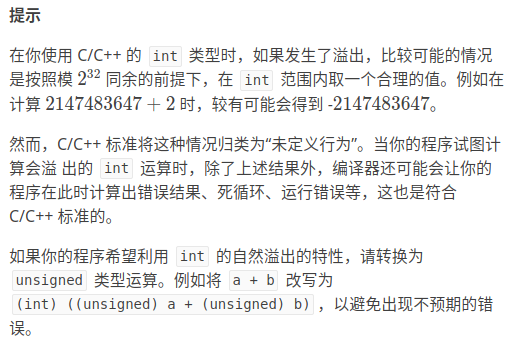
\includegraphics[scale = 0.5]{figures/from-luogu.png}
    \end{figure}
\end{frame}

\begin{frame}[fragile]{Infinite Loops}
    \ttt{while (true)} + \ttt{break} can be used as substitute for \ttt{do}-\ttt{while} loops.
    \begin{columns}
        \column{0.5\textwidth}
        \begin{cpp}
// Why is n declared here?
int n;
do {
  scanf("%d", &n);
  if (n < 0)
    printf("Please input again!\n");
} while (n < 0);
        \end{cpp}
        \column{0.5\textwidth}
        \begin{cpp}
while (true) {
  int n;
  scanf("%d", &n);
  if (n < 0)
    printf("Please input again!\n");
  else
    break;
}
        \end{cpp}
    \end{columns}
\end{frame}

\begin{frame}[fragile]{\ttt{break} vs \ttt{continue}}
    Explain the behavior of the following code.
    \begin{cpp}
for (int i = 0; i < n; ++i) {
  if (a[i] % 2 == 1)
    continue;
  int x = calc(a[i]);
  if (check(x))
    break;
  update(a[i]);
  ++count;
}
    \end{cpp}
\end{frame}

\begin{frame}[fragile]{\ttt{break} vs \ttt{continue}}
    Explain the behavior of the following code.
    \begin{cpp}
for (int i = 0; i < n; ++i) {
  if (a[i] % 2 == 1)
    continue;
  int x = calc(a[i]);
  if (check(x))
    break;
  update(a[i]);
  ++count;
  // `continue' goes here.
}
// `break' goes here.
    \end{cpp}
\end{frame}

\begin{frame}[fragile]{Variable Declaration in \ttt{switch}-\ttt{case}}
    Due to the special control path of \ttt{switch}-\ttt{case} statements, any \ttt{case} branch that contains a variable declaration must be a block.
    \begin{cpp}
switch (a) {
  case 1: {
    int x = calc(a);
    // do something
    break;
  }
  case 2:
    // x cannot be used here.
    break;
  default:
    break;
}
    \end{cpp}
\end{frame}

\section{Arrays and Pointers}

\begin{frame}[fragile]{Constant Expressions}
	\begin{itemize}
		\item \blue{Constant expressions} refer to the expressions that can be evaluated \blue{during compile-time}.
		\item In C:
		\begin{itemize}
			\item Expressions that only contain literals
			\item \red{\ttt{enum} hack}
		\end{itemize}
		\pause
		\item \ttt{\#define PI 3.14}\\
		Is \ttt{PI} a constant expression?\\
		\pause
		\blue{Yes, because \ttt{PI} will be replaced by the literal \ttt{3.14}.}
		\pause
		\item \ttt{const int maxn = 100;}\\
		Is \ttt{maxn} a constant expression?\\
		\pause
		\blue{No. \ttt{maxn} is a constant variable.}
	\end{itemize}
\end{frame}

\begin{frame}[fragile]{Constant Expressions}
	The value of \ttt{const} variables cannot be changed after initialization, but may not be determined during compile time.
	\begin{cpp}
int i;
scanf("%d", &i);
const int j = i;
	\end{cpp}
	\pause
	\begin{itemize}
		\item \bluett{const} variables initialized with a constant expression is also constant expression \red{in C++, but not in C}.
		\item \bluett{const }\ttt{int maxn = 100;} is a constant expression in C++, but not in C.
	\end{itemize}
\end{frame}

\begin{frame}[fragile]{\ttt{enum} Hack}
	\begin{cpp}
enum { maxn = 100 };
int a[maxn];
	\end{cpp}
	\begin{itemize}
		\item \ttt{maxn} has type \ttt{int}, and it is a constant expression.
		\pause
		\item Use \ttt{enum} hack to define \ttt{bool}:
		\begin{cpp}
typedef enum { false, true } bool;
		\end{cpp}
		\item[\(\Rightarrow\)] \textit{Effective C++}, Item 2.
	\end{itemize}
\end{frame}

\begin{frame}[fragile]{Define an Array}
	\ttt{type name[N];}
	\begin{itemize}
		\item \ttt{N} \textbf{must be a constant expression}. (We will talk about this later.)
		\item The following code is illegal \red{before C99}, even though many compilers are so smart that they can handle it.
		\begin{cpp}
const int maxn = 1000;
int a[maxn]; // Error: maxn is not a constant expression.
		\end{cpp}
	\end{itemize}
\end{frame}

\begin{frame}{Element Access}
	\begin{itemize}
		\item Access through \blue{subscript}: \ttt{a[i]}.
		\pause
		\item \ttt{*(a + i)}: an equivalent way, but treats array as a pointer.
		\item In fact, subscript operator also works on pointers: \ttt{p[i]} is the same as \ttt{*(p + i)} for a pointer \ttt{p}.
		\pause
		\item What does \ttt{scanf("\%d", a + i)} mean?\\
		\pause
		\blue{Same as \ttt{scanf("\%d", \&a[i])}.}
	\end{itemize}
\end{frame}

\begin{frame}[fragile]{Traversal}
	\begin{itemize}
		\item Through subscript:
		\begin{cpp}
for (int i = 0; i < n; ++i)
  do_something(a[i]);
		\end{cpp}
		\item Through pointer:
		\begin{cpp}
for (int *p = a, *end = a + n; p != end; ++p)
  do_something(*p);
		\end{cpp}
		\pause
		\item More fancy way:
		\begin{cpp}
int *p = a, *end = a + n;
while (p != end)
  do_something(*p++);
		\end{cpp}
	\end{itemize}
\end{frame}

\begin{frame}[fragile]{The '\ttt{*}' Specifier}
	Use '\ttt{*}' to define a pointer.
	\begin{itemize}
		\item Both \ttt{int *p} and \ttt{int* p} are right,
		\pause
		\item but the latter may fool you in some cases:
		\begin{cpp}
int* p1, p2, p3;
		\end{cpp}
		\pause
		\item Choose one way and persist. If you choose \ttt{int* p}, never define more than one pointers in one declaration!
	\end{itemize}
\end{frame}

\begin{frame}[fragile]{Confusing Types}
	\begin{itemize}
		\item \ttt{int (*a)[10]}: \ttt{a} is a pointer, which points to an array, which stores \ttt{10} \ttt{int}s.
		\item \ttt{int *a[10]}: \ttt{a} is an array, which stores \ttt{10} pointers, each pointing to an \ttt{int}.
		\pause
		\item Use type alias:
		\begin{cpp}
typedef int arr_t[10];
arr_t *a;
typedef int *ptr_t;
ptr_t pa[10];
		\end{cpp}
	\end{itemize}
\end{frame}

\begin{frame}{Constant Types}
	\begin{itemize}
		\item \bluett{const }\ttt{int *p} and \ttt{int }\bluett{const }\ttt{*p} are the same: a pointer, which points to a \bluett{const} \ttt{int}.
		\item \ttt{int *}\bluett{const }\ttt{p}: a constant variable, which is a pointer, which points to an \ttt{int}.
		\pause
		\item When a variable itself is constant, it is a \blue{top-level const}. When a variable is a pointer that points to a constant variable, it is a \blue{low-level const}.
		\item \bluett{const }\ttt{int *}\bluett{const }\ttt{p} is both top-level const and low-level const.
	\end{itemize}
\end{frame}

\begin{frame}[fragile]{\bluett{const} and Pointers}
	\begin{itemize}
		\item Low-level const pointers can point to non-const variables, which is called `\textbf{adding low-level const}'.
		\begin{cpp}
int i = 42;
const int *p = &i;
		\end{cpp}
		\item Modifying \ttt{i} through \ttt{p} is not allowed, but it can be modified in other ways.
		\pause
		\item \textbf{Deleting low-level const} is not allowed:
		\begin{cpp}
int *p2 = p; // Error
		\end{cpp}
		\pause
		\item[\(\Rightarrow\)] \textit{Effective C++}, Item 3.
	\end{itemize}
\end{frame}

\begin{frame}{Multi-dimensional Arrays}
	There's no so-called \blue{multi-dimensional} arrays in C/C++. Instead, they are \blue{arrays of arrays}.
	\begin{itemize}
		\item \bluett{int }\ttt{a[3][4];} `\ttt{a}' is an array of size \ttt{3}, where each element is an array of 4 \bluett{int}s.
		\pause
		\item Storage of 2d-array: \red{Not} a matrix!
		\begin{figure}[h]
			\centering
			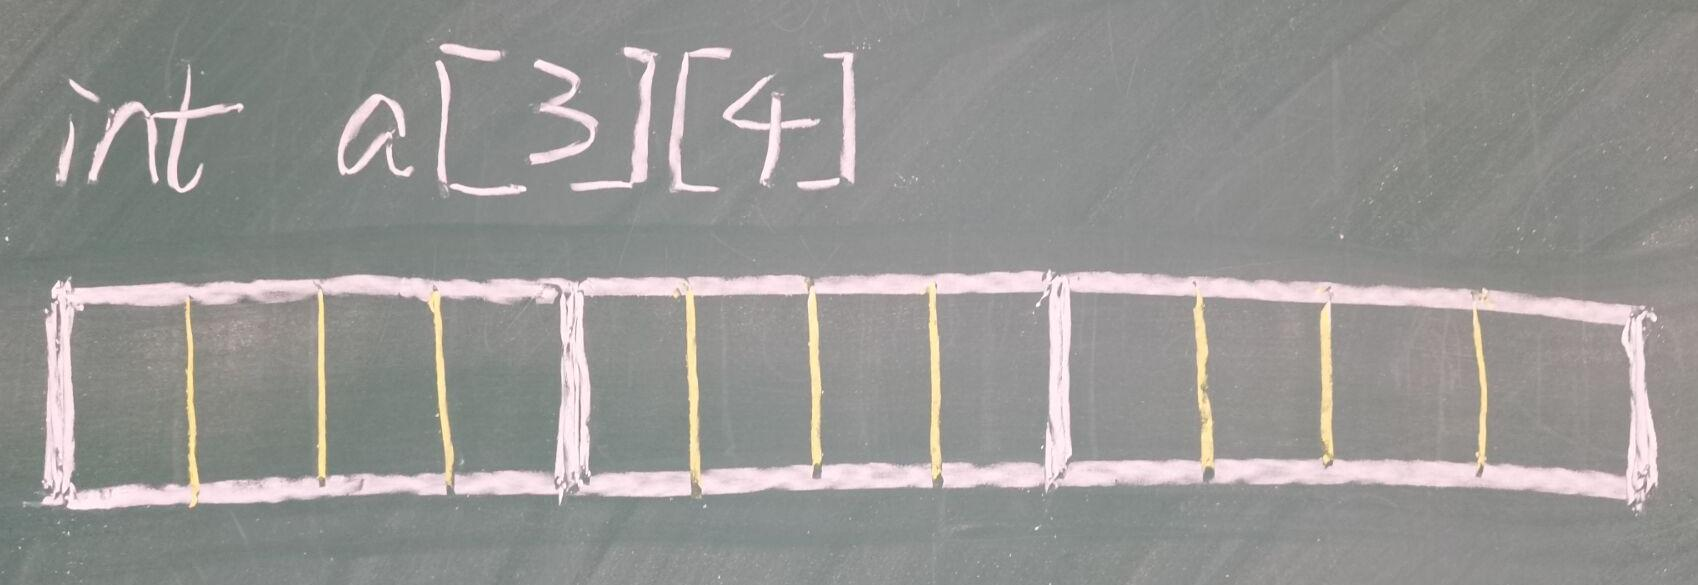
\includegraphics[scale=0.2]{figures/2darray.jpg}
		\end{figure}
	\end{itemize}
\end{frame}

\begin{frame}{\ttt{size\_t} and \ttt{ptrdiff\_t}}
	Defined in header \ttt{stddef.h}.
	\begin{itemize}
		\item \ttt{size\_t} is an \blue{unsigned} integer type of the result of \bluett{sizeof}.
		\item \ttt{size\_t} can store the maximum size of a theoretically possible object of any type.
		\item \ttt{ptrdiff\_t} is a \blue{signed} integer type of the result of subtracting two pointers.
		\item Both \ttt{size\_t} and \ttt{ptrdiff\_t} are \red{implementation-defined}.
	\end{itemize}
\end{frame}

\begin{frame}{Variable Length Array}
	\begin{itemize}
		\item Since C99, the length of arrays is allowed to be determined during runtime.
		\item Since C11, compilers may define the macro \bluett{\_\_STDC\_NO\_VLA\_\_} to integer \ttt{1} to indicate that VLA is not supported.
		\item VLA is constructed on \blue{stack}, while the `dynamic-arrays' allocated by \ttt{malloc} are on \blue{heap}.
		\pause
		\item \textbf{VLA has never been supported by standard C++.}
		\item We do not recommend to use VLA. Instead, use dynamic memory when the length of array is determined during runtime.
		\item \url{https://en.cppreference.com/w/c/language/array}
	\end{itemize}
\end{frame}

\section{Functions}

\begin{frame}{Declaration vs Definition}
	\begin{itemize}
		\item Declaration without definition:\\
		\ttt{return-type function-name(params);}
		\item Definition:\\
		\ttt{return-type function-name(params) \{function-body\}}\\
		There is \red{no semicolon} at the end of function definition!
		\pause
		\item A function can be declared any times, but only defined once.
		\item A definition is also a declaration.
		\item There should be at least one declaration of the function before it is called.
		\item In a declaration, the names of the parameters can be omitted, as they are not used.
	\end{itemize}
\end{frame}

\begin{frame}[fragile]{Calling a Function}
	\begin{cpp}
int factorial(int n) {
  int s = 1;
  for (int i = 1; i <= n; ++i)
    s *= i;
  return s;
}
int main() {
  int n;
  scanf("%d", &n);
  printf("%d\n", factorial(n));
  return 0;
}
	\end{cpp}
\end{frame}

\begin{frame}[fragile]{Calling a Function}
	\bluett{int }\ttt{result = factorial(n);}
	\begin{itemize}
		\item The `\bluett{()}' is called the \blue{function-call operator}.
		\item The function-call operator \red{cannot be omitted}, even if the function takes no arguments.
		\pause
		\item Statements that do nothing:
		\begin{cpp}
;
5;
2 + 3;
{}
n;
fun;
		\end{cpp}
	\end{itemize}
\end{frame}

\begin{frame}[fragile]{Passing Arrays to Functions}
	Define an array parameter:
	\begin{itemize}
		\item \ttt{int *a}, \ttt{int a[]} and \ttt{int a[n]} are \textbf{totally the same}: array types \blue{decay} to pointer types.
		\pause
		\item C functions have no way of knowing the length of an array parameter.
		\item C functions cannot require the array parameter to be of any certain length. (They cannot even require it to be an array!)
		\pause
		\item The following code compiles, but may cause disaster.
		\begin{cpp}
void fun(int a[10]) {}
int i;
fun(&i);
		\end{cpp}
	\end{itemize}
\end{frame}

\begin{frame}[fragile]{Passing Arrays to Functions}
	Example:
	\begin{cpp}
void print_array(int *a, int n) {
  for (int i = 0; i < n; ++i)
    printf("%d ", a[i]);
}
int main() {
  int arr[] = {2, 5, 6};
  print_array(arr, 3);
  return 0;
}
	\end{cpp}
\end{frame}

\begin{frame}[fragile]{Passing Arrays to Functions}
	\begin{cpp}
void print_array2(int *begin, int *end) {
  for (int *p = begin; p != end; ++p)
    printf("%d ", *p);
}
void print_array3(int *begin, int *end) {
  while (begin != end)
    printf("%d ", *begin++);
}
int main() {
  int arr[] = {2, 5, 6};
  print_array2(arr, arr + 3);
  print_array3(arr, arr + 3);
  return 0;
}
	\end{cpp}
\end{frame}

\begin{frame}[fragile]{Passing Multi-dimensional Arrays to Functions}
	\begin{itemize}
		\item What type will \ttt{int [3][4]} decay to?\\
		\pause
		\blue{\ttt{int [3][4]} is an array of \ttt{int [4]}, so it will decay to a pointer that points to \ttt{int [4]}}, that is:\\
		\ttt{int (*)[4]}
		\pause
		\item Differentiating \ttt{int (*a)[4]} and \ttt{int *a[4]}.\\
		\blue{\ttt{int (*a)[4]} is a pointer that points to \ttt{int [4]},\\
		while \ttt{int *a[4]} is an array of four pointers, each pointing to an \ttt{int}.}
	\end{itemize}
\end{frame}

\begin{frame}[fragile]{Passing Muldi-dimensional Arrays to Functions}
	\begin{cpp}
void print_2darray(int (*a)[4], int n) {
  for (int i = 0; i < n; ++i) {
    for (int j = 0; j < 4; ++j)
      printf("%d ", a[i][j]);
    puts("");
  }
}
int main() {
  int a[3][4] = /* some value */;
  print_2darray(a, 3);
  return 0;
}
	\end{cpp}
	The size `4' cannot be left out, otherwise it will become an \blue{incomplete type} (\ttt{int (*)[]}).
\end{frame}

\begin{frame}[fragile]{Safety Issue of \ttt{scanf}}
	Use \ttt{scanf} to read a string:
	\begin{cpp}
char str[100];
scanf("%s", str);
	\end{cpp}
	\pause
	\begin{itemize}
		\item \ttt{scanf} has no idea how big your array is!
		\item \textbf{Array subscript out of range} is severe runtime error, which cannot be detected during compile-time, and may not report when happening. (On Linux systems, it reports a `segmentation fault'.)
		\pause
		\item Functions like \ttt{gets} are removed in modern C and C++ due to similar issues. Functions like \ttt{scanf\_s} are introduced for safety.
	\end{itemize}
\end{frame}

\begin{frame}[fragile]{Modifying Outer Variables}
	The following definition of a `swap' function does not work:
	\begin{cpp}
void swap(int a, int b) {
  int tmp = a;
  a = b;
  b = tmp;
}
	\end{cpp}
	\pause
	Because \ttt{a} and \ttt{b} are local variables of the function.\\
	When \ttt{swap(x, y)} is called, the variables \ttt{a} and \ttt{b} are initialized with values of \ttt{x} and \ttt{y} respectively. In other words, they are \blue{copies} of \ttt{x} and \ttt{y}.
\end{frame}

\begin{frame}[fragile]{Modifying Outer Variables}
	Pass by pointer:
	\begin{cpp}
void swap(int *a, int *b) {
  int tmp = *a;
  *a = *b;
  *b = tmp;
}
	\end{cpp}
	\pause
	\begin{question}
		Why is `\ttt{\&}' needed when passing a variable to \ttt{scanf}, but not needed for \ttt{printf}?
	\end{question}
\end{frame}

\begin{frame}[fragile]{Returning Multiple Values}
	As in HW2-1:
	\begin{cpp}
void findSecondMaxAndMin(int a[], int size, int *secondMin, int *secondMax) {
  *secondMin = /* some value */;
  *secondMax = /* some value */;
}
	\end{cpp}
	\pause
	Can we write as in \ttt{Python}?
	\begin{cpp}
return (secondMin, secondMax);
	\end{cpp}
\end{frame}

\begin{frame}[fragile]{The Comma Operator}
	\begin{itemize}
		\item The comma in the expression `\ttt{a, b}' is the \blue{comma operator}. It is the operator of \blue{the lowest precedence}.
		\pause
		\item The evaluation order is determined! \blue{(4)}
		\item The left operand is evaluated first, and then the right operand is evaluated.
		\item The return value of the comma expression is the value of the right operand.
		\begin{cpp}
// a is initialized with value of c.
int a = (b, c);
		\end{cpp}
		\pause
		\item Not all commas are \blue{comma operators}. Some work as a part of the grammar.
	\end{itemize}
\end{frame}

\begin{frame}[fragile]{Function Inlining}
	\begin{cpp}
#define MAX(A, B) ((A) < (B) ? (B) : (A))
	\end{cpp}
	Pros and cons?
	\pause
	\begin{itemize}
		\item Time- and memory-saving, in comparison with functions.
		\item May cause unexpected results:
		\begin{cpp}
int x = MAX(++i, j);
		\end{cpp}
		\pause
		\item We want the compiler to expand the function at the \blue{call site} instead of calling it, so that the time and memory cost could be reduced.
	\end{itemize}
\end{frame}

\begin{frame}[fragile]{Function Inlining}
	\begin{cpp}
inline double max(double a, double b) {
  return a < b ? b : a;
}
	\end{cpp}
	\begin{itemize}
		\item The \bluett{inline} specifier is a hint for the compiler to perform inline expansion.
		\item Compilers have the right to accept or ignore the \bluett{inline} specifier.
		\pause
		\item Usually, inline request will be accepted for simple and short functions,
		\item and ignored for functions that are \blue{too long} or \blue{recursive}.
		\pause
		\item Function inlining are not without drawbacks.
		\item[\(\Rightarrow\)] \textit{Effective C++}, Item 30.
	\end{itemize}
\end{frame}

\end{document}